\documentclass{standalone}
\usepackage{tikz}
\usepackage{amsmath}
\renewcommand{\familydefault}{\sfdefault}


\begin{document}

\def\d{6.5}
\def\q{-8}
\begin{tikzpicture}
    \node at (0*\d, 0) {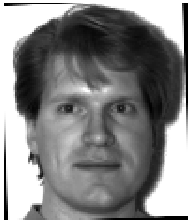
\includegraphics{../python/ori01.png}};
    \node at (1*\d, 0) {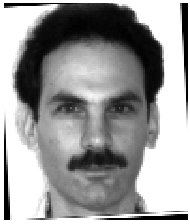
\includegraphics{../python/ori02.png}};
    \node at (2*\d, 0) {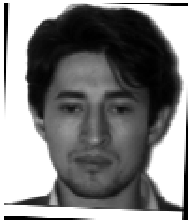
\includegraphics{../python/ori03.png}};
    \node at (3*\d, 0) {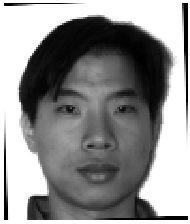
\includegraphics{../python/ori04.png}};
    \node at (4*\d, 0) {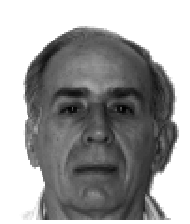
\includegraphics{../python/ori05.png}};
    \node at (5*\d, 0) {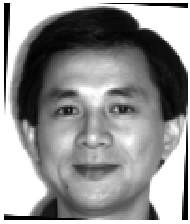
\includegraphics{../python/ori06.png}};


    \node at (0*\d, \q) {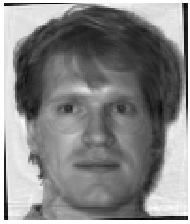
\includegraphics{../python/res01.png}};
    \node at (1*\d, \q) {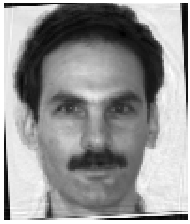
\includegraphics{../python/res02.png}};
    \node at (2*\d, \q) {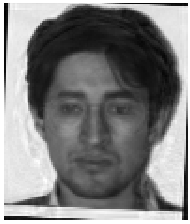
\includegraphics{../python/res03.png}};
    \node at (3*\d, \q) {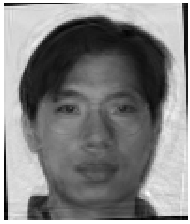
\includegraphics{../python/res04.png}};
    \node at (4*\d, \q) {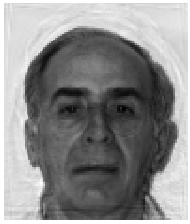
\includegraphics{../python/res05.png}};
    \node at (5*\d, \q) {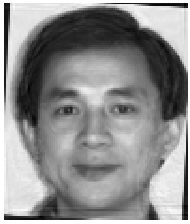
\includegraphics{../python/res06.png}};

    % \node at (0*\d, 2*\q) {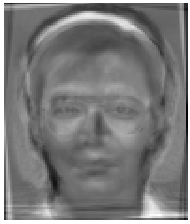
\includegraphics{../python/eigenface12.png}};
    % \node at (1*\d, 2*\q) {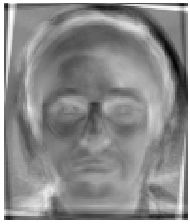
\includegraphics{../python/eigenface13.png}};
    % \node at (2*\d, 2*\q) {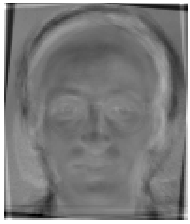
\includegraphics{../python/eigenface14.png}};
    % \node at (3*\d, 2*\q) {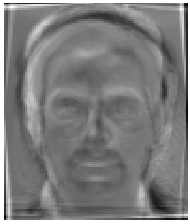
\includegraphics{../python/eigenface15.png}};
    % \node at (4*\d, 2*\q) {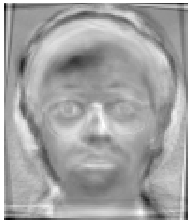
\includegraphics{../python/eigenface16.png}};
    % \node at (5*\d, 2*\q) {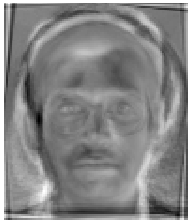
\includegraphics{../python/eigenface18.png}};

\end{tikzpicture}
% End of code
\end{document}
